\section{Analysis Strategy}
%%%%%%%%%%%%%%%%%%%%%%%%%%%%%%%%%%%%%%%%%%%%%%%%%%%%%%%%%%%%%%%%%%%%%%
\label{sec:AnalysisStrategy}

The analysis presented here is based on that used in the previously published \hwwllnn
measurements by CMS~\cite{Chatrchyan:2013iaa}, modified to be inclusive in the number of jets. 
This modification significantly reduces the uncertainties related to the modelling of the number of jets produced in association with the Higgs boson.

The signal contribution is extracted performing a template binned likelihood fit, using the two-dimensional (\mll,\mt) shape for each background and signal process, as described in Sec.~\ref{sec:SignalExtraction}.

The \mll variable represents the invariant mass of the two leptons in the event while \mt is the invariant transverse mass of the final state objects, and is defined as follows:
\begin{equation}
\mt = \sqrt{2\ptll\MET(1-\cos\Delta\phi(\vec{p}_\mathrm{T}^{~\ell\ell},\ptmiss))} \quad ,
\end{equation}
\noindent where $\vec{p}_\mathrm{T}^{~\ell\ell}$ is the dilepton transverse momentum vector and $\Delta\phi(\vec{p}_\mathrm{T}^{~\ell\ell},\ptmiss)$ the azimuthal angle between $\vec{p}_\mathrm{T}^{~\ell\ell}$ and \ptmiss.

\subsection{Event reconstruction and selections}\label{sec:Selections}

Electrons and muons used in the analysis are reconstructed using the PF technique as described in Sec.~\ref{sec:leptonID}. In particular, muon candidates are required to be identified both as Tracker Muons and Global Muons.

Jets are reconstructed using the standard PF algorithm and using the anti-$k_t$ clustering algorithm with $\mathrm{R} = 0.5$, as described in Sec.~\ref{sec:jets}. Unless specified otherwise, jets considered for jet counting are the ones with $\pt > 30$\,\GeV.

In addition to the standard CMS PF \MET, a \textit{projected} \MET variable is also used. The \textit{projected} \MET is defined as the component of \ptmiss transverse to the nearest lepton if the lepton is situated within the azimuthal angular window of $\pm \pi/2$ from the \ptmiss direction, or the \MET itself otherwise.
Since the \MET resolution is degraded by pile-up, the minimum of two projected \MET variables is used: one constructed from all identified particles (full projected \MET), and another constructed from the charged particles only (track projected \MET).

Background events from \ttbar and tW production are rejected applying a soft-muon veto and a b tagging veto. The soft-muon algorithm is designed to identify muons from b quark decays requiring loose muon identification selections, as described in Sec.~\ref{sec:muID}, and low relative isolation (greater than 0.1 for muons with $\pt>20$\GeV). Events containing at least one muon satisfying these requirements are rejected by the soft-muon veto.

The b tagging veto rejects events that contain jets identified as b-jets using two different algorithms for high and low \pt jets (see Sec.~\ref{sec:btag}). For jets with \pt between 10 and 30\GeV, the TCHE algorithm is used. Low-\pt jets passing the TCHE discriminant threshold of 2.1 are tagged as b-jets.
For jets with $\pt>30$\GeV, a better performing algorithm, JP, is used. Jets are identified as b-jets by the JP algorithm if the discriminating variable has a value above 1.4.
In the following, a b-tagged jet is defined as a jet, within $|\eta|<2.4$ (b tagging requires the tracker information), and with a value of the discriminating variable above the mentioned thresholds for the two algorithms.

The event selection consists of several steps. The first step is to select \WW-like events applying a selection that consists of the following set of cuts:
\begin{itemize}
\item {\bf Lepton preselection}:
  \begin{itemize}
  \item two opposite charge and different flavour (e$\mu$) isolated leptons reconstructed in the event;
  \item $|\eta|<2.5$ for electrons and $|\eta|<2.4$ for muons;
  \item $\pt>20\GeV$ for the leading lepton. For the trailing lepton, the transverse momentum is required to be larger than 10\GeV;
  \end{itemize}
\item {\bf Extra lepton veto}: the event is required to have two and only two leptons passing the lepton selection;
\item {\bf \boldmath$\MET$ preselection}: particle flow \MET is required to be greater than 20\GeV;
\item {\bf Projected \boldmath$\MET$ selection}: minimum projected \MET is required to be larger than 20\GeV;
\item {\bf Dilepton mass cut}: $\mll > 12$\GeV in order to reject low mass resonances and multijet backgrounds;
\item {\bf Dilepton \boldmath$\pt$ cut}: $\ptll > 30$\GeV to reduce the contribution of W+jets and \dytt backgrounds;
\item {\bf Transverse mass}: $\mt>60$\GeV to reject \dytt events. 
\end{itemize}
The requirement of different flavour leptons in the final state is important in order to suppress the sizeable contribution of backgrounds containing a same flavour lepton pair originating from Z boson decay.

Events surviving these requirements are dominantly those where a top quark-antiquark pair is produced and both W bosons, which are part of the top quark decay chain, decay leptonically (dileptonic \ttbar).
Two different selections are used depending on the number of jets in the event. This is done to suppress the top quark background both in the low \pth region, where 0 jets events have the largest contribution, and for higher \pth values where also larger jet multiplicity events are important.
The selection for 0 jets events relies on the soft-muon veto and on a soft jet (with $\pt < 30$\GeV) b tagging veto.
The latter requirement exploits the TCHE algorithm to reject soft jets that are likely to come from b quarks hadronization.

For events with a jet multiplicity greater or equal than one a different selection is applied. In this case the good b tagging performances of the JP algorithm is exploited to reject events containing jets with $\pt > 30$\GeV that are likely to come from b quarks hadronization. The analysis selection requires to have no events containing b-tagged jets with $\pt > 30$\GeV.

\begin{figure}[htb]
\centering
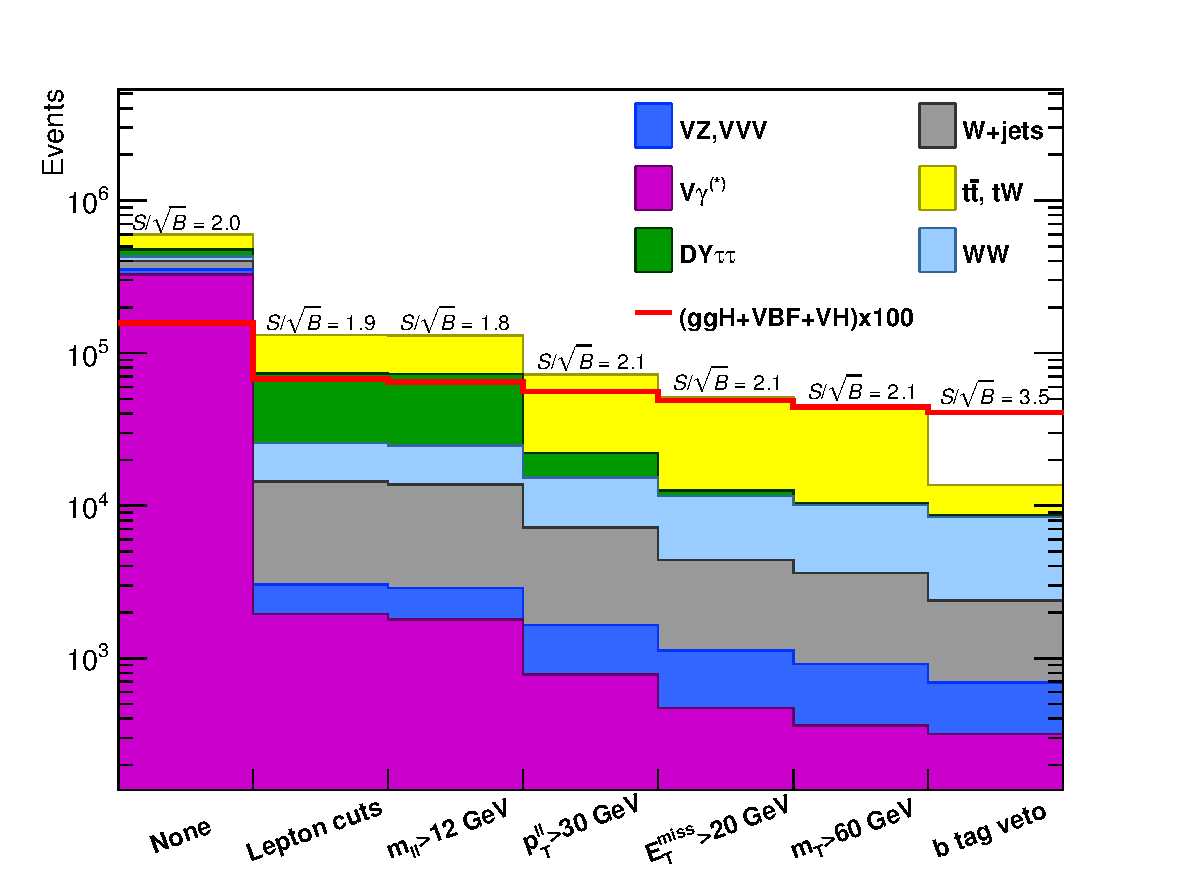
\includegraphics[width=0.8\textwidth]{images/cutflow-thesis.pdf}
\caption{Effect of selection cuts on simulated samples. The signal (red line) is multiplied by 100 and superimposed on stacked backgrounds. In each bin, corresponding to a different selection, the expected number of events in MC at a luminosity of $19.46~\mathrm{fb}^{-1}$ is shown.}\label{fig:cutflow}
\end{figure}

A cut-flow plot is shown in Fig.~\ref{fig:cutflow}, illustrating the effect of each selection using signal and background simulations. In the first bin, labelled as ``No cut'', only a very loose selection is applied and the bin content corresponds to the total expected number of events with a luminosity of $19.4~\mathrm{fb}^{-1}$. All the events in this bin have at least two leptons with a loose transverse momentum cut of 8\GeV. In the following bin the lepton cuts are applied, including the requirement to have two opposite sign and different flavour leptons and the extra lepton veto. Then all the other selections are progressively reported, showing the effect of each cut on the background and signal yields. For each selection the expected significance ($S/\sqrt{B}$) is also shown, which, after the full selection requirements, reaches a maximum value of about 3.5. The expected significance is computed neglecting all sources of uncertainties.


\subsection{Simulation efficiencies and scale factors}\label{sec:ScaleFactors}
The efficiencies for the identification and isolation of electrons and muons are measured in data and simulation selecting a pure sample of leptons coming from the $\mathrm{Z\to\ell\ell}$ decay, and using the Tag and Probe technique described in Sec.~\ref{sec:lepIdIsoEff}. The efficiencies for data and simulation are used as scale factors to correct the simulated events to precisely model the data.

The trigger efficiency is measured in data and applied to simulation as explained in Sec.~\ref{sec:trigeff}.

The efficiency of b tagging algorithms is not well simulated by MC generators and discrepancies may occur with respect to the data. For this reason is important to measure the b tagging efficiency and the misidentification probability for the given algorithms both in data and simulation, and to correct the simulated events using scale factors. This affects not only the top quark background estimation, but also other backgrounds and signal. As an example, if a light-parton jet in a signal event was misidentified as a b-jet, this event would be rejected by the b-jet veto.

In this analysis, the b tagging efficiency and the misidentification probability are measured both in data and simulation, selecting a control sample enriched in b-jets, and using a Tag and Probe technique similar to the one described in Sec.~\ref{sec:lepIdIsoEff}. The method used to estimate the efficiency of the JP b tagging algorithm is described below, but this method is extendible to any other algorithm.

The control sample is defined selecting events that pass the selections listed in Sec.~\ref{sec:Selections}, and have at least two jets with \pt greater than 30\GeV. If the leading jet has a JP discriminator value above the threshold of 0.5 it is considered a \emph{tag}, and the subleading jet is the \emph{probe}. In order to avoid any bias that could arise from the probe being always the subleading jet, the pair is tested also in reverse order, i.e. subleading jet is tested against the \emph{tag} selection, and in case it passes, the leading jet is used as \emph{probe} forming an independent \emph{tag-probe} pair. If the \probe jet has a discriminator value above the threshold used in the analysis, i.e. $>1.4$, then the \tp pair is called a \tpp pair. Otherwise it is identified as a \tfp pair.

If the \tg selection was sufficient to suppress any non top quark event, one could estimate the efficiency by dividing the number of \tp pairs in which the \probe passes the analysis JP requirement by the total number of \tp pairs. However this is not the case, since the contamination due to other background sources is not negligible. In order to estimate the efficiency in the presence of background, a variable that discriminates between true b-jets and other jets in a \ttbar sample is needed. This variable is the \pt of the \probe jet. For real b-jets this variable has a peak around 60\GeV, while it has a broad distribution for other types of jets.

The efficiencies are estimated performing a $\chi^{2}$ simultaneous fit of the \probe \pt spectrum in two different categories: one containing events with a \tpp pair and the other containing events with a \tfp pair. The normalisations in the two categories are linked by the following formulas:
\begin{equation}
\begin{split}
N_\mathrm{TPP} &= N_\mathrm{s} \varepsilon_\mathrm{s} + N_\mathrm{b} \varepsilon_\mathrm{b} \\
N_\mathrm{TFP} &= N_\mathrm{s} (1 -\varepsilon_\mathrm{s}) + N_\mathrm{b} ( 1 - \varepsilon_\mathrm{b}) \quad,
\end{split}
\end{equation}
\noindent where:
\begin{itemize}
\item $N_\mathrm{TPP}$ is the number of \tpp pairs;
\item $N_\mathrm{TFP}$ is the number of \tfp pairs;
\item $N_\mathrm{s}$ is the number of \tp pairs in which the \probe is a b-jet\footnote{In these naming convention, the subscript ``s'' stays for ``signal'', since the b-jets represent the signal in this case. Similarly, the ``b'' subscript stays for ``background'', identifying the cases where the \probe is not a b-jet};
\item $N_\mathrm{b}$ is the number of \tp pairs in which the \probe is not a b-jet;
\item $\varepsilon_\mathrm{s}$ is the efficiency to identify a b-jet, i.e. the b tagging efficiency;
\item $\varepsilon_\mathrm{b}$ is the probability to misidentify a non b-jet as a b-jet, i.e. the misidentification probability.
\end{itemize}

\begin{figure}[!htb]
\centering
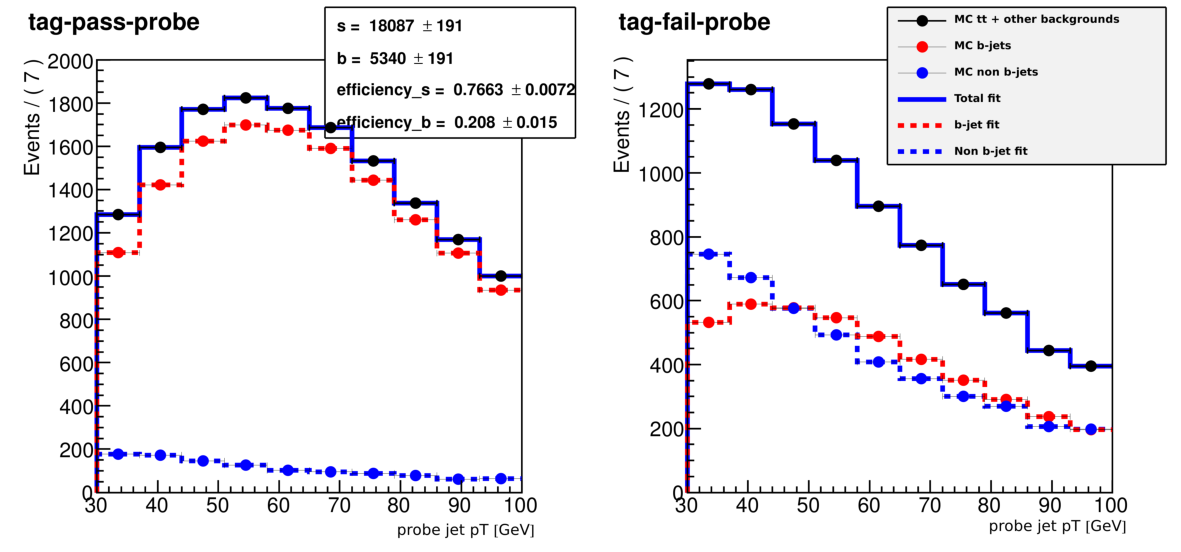
\includegraphics[width=0.8\textwidth]{images/mc_pt_probe-v2.pdf}
\caption{Results of the simultaneous fit of the \tpp and \tfp pairs in the MC simulation.\label{fig:mc_tp}}
\end{figure}

The \pt shapes of the \probe jet used in the fit are taken from simulation, where the real flavour of the jet is known, both for the \tpp and \tfp categories. To check the consistency of the fitting procedure a closure test fitting the simulation itself is performed.
The result of the fit on MC simulation is shown in Fig.~\ref{fig:mc_tp}. The relevant efficiencies are:
\begin{equation}
\begin{split}
\varepsilon_\mathrm{s}^\mathrm{MC} &= 0.766\pm0.007 \\
\varepsilon_\mathrm{b}^\mathrm{MC} &= 0.208\pm0.015 \quad .
\end{split}
\end{equation}
These values are consistent with the true value of the b tagging efficiency in simulation. The true value is computed by selecting jets that are matched within a cone of $\Delta{R}<0.5$ with a generator level b quark, and counting the fraction of those that have a JP discriminator above the threshold of 1.4. This check also assures that the \tp method does not introduce any bias within the simulation statistic accuracy.

\begin{figure}[htb]
\centering
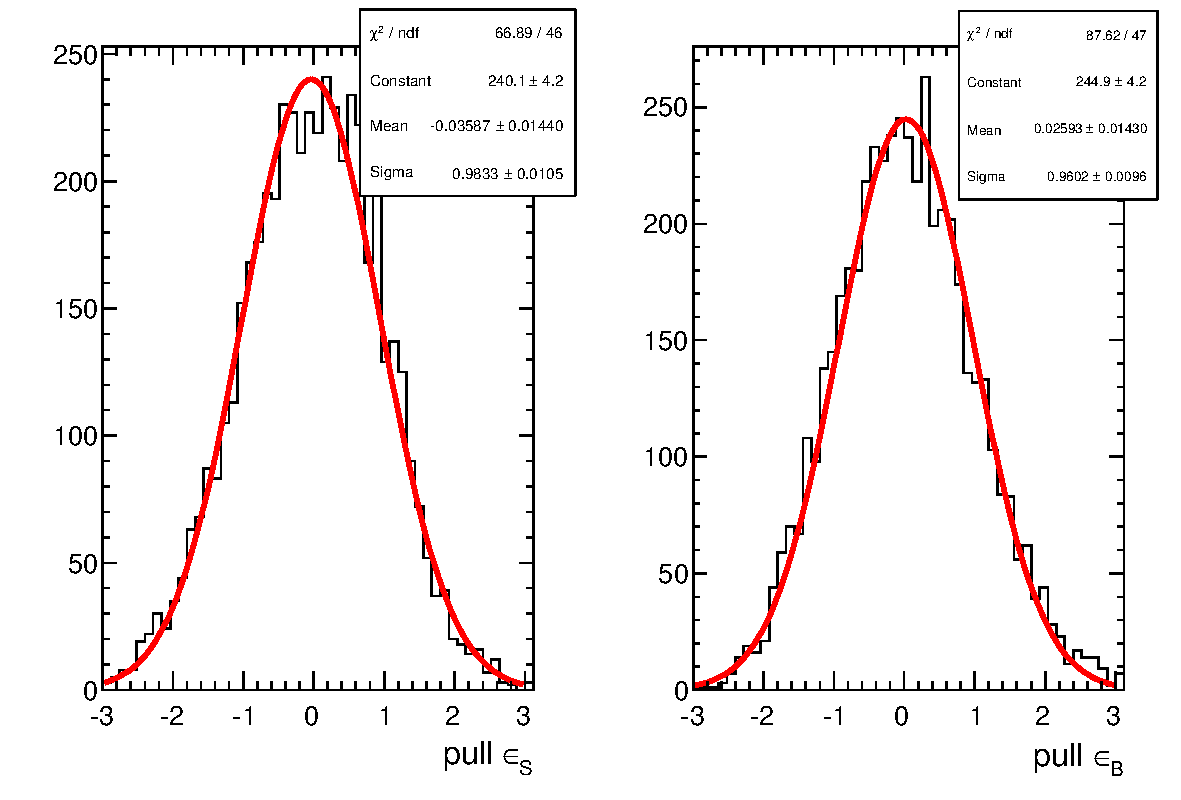
\includegraphics[width=0.7\textwidth]{images/pulls_mc.pdf}
\caption{Pulls distribution for the $\varepsilon_{\rm s}$ and $\varepsilon_{\rm b}$ efficiencies obtained with MC toy simulations.\label{fig:pullstp}}
\end{figure}

In order to assess the robustness of the fit, 5000 toy simulated samples have been generated with a statistics equivalent to the one expected in data and the same fit is performed for each of them. All the 5000 fit succeeded, and the pull distributions for $\varepsilon_{\rm s}$ and $\varepsilon_{\rm b}$ parameters are shown in Fig.~\ref{fig:pullstp}. The pull variable for each toy $i$ is defined as:
\begin{equation}
pull(\varepsilon_{\rm s (b)}) = \frac{\varepsilon_{\rm s (b)}^{\rm true} - \varepsilon_{\rm s (b)}^{i}}{\sigma(\varepsilon_{\rm s (b)}^{i})} \quad,
\end{equation}
\noindent where $\sigma(\varepsilon_{\rm s (b)}^{i})$ is the uncertainty on the efficiency extracted from the fit. The pull distributions are centred on zero and have $\sigma$ close to one, as expected.

Before running the fit on data, the shapes used in the fit have been validated. To do so, a very pure phase space enriched in b-jets is defined by selecting events containing exactly two jets with a JP discriminator greater than 1.5 and no additional b-tagged jet, rejecting also events containing jets with \pt smaller than 30 \GeV. On this very pure sample, data have been compared against the shape used to fit the true b-jets in the \tpp distribution. The result is shown in Fig.~\ref{fig:purett} and shows good agreement within uncertainties.

\begin{figure}[htb]
\centering
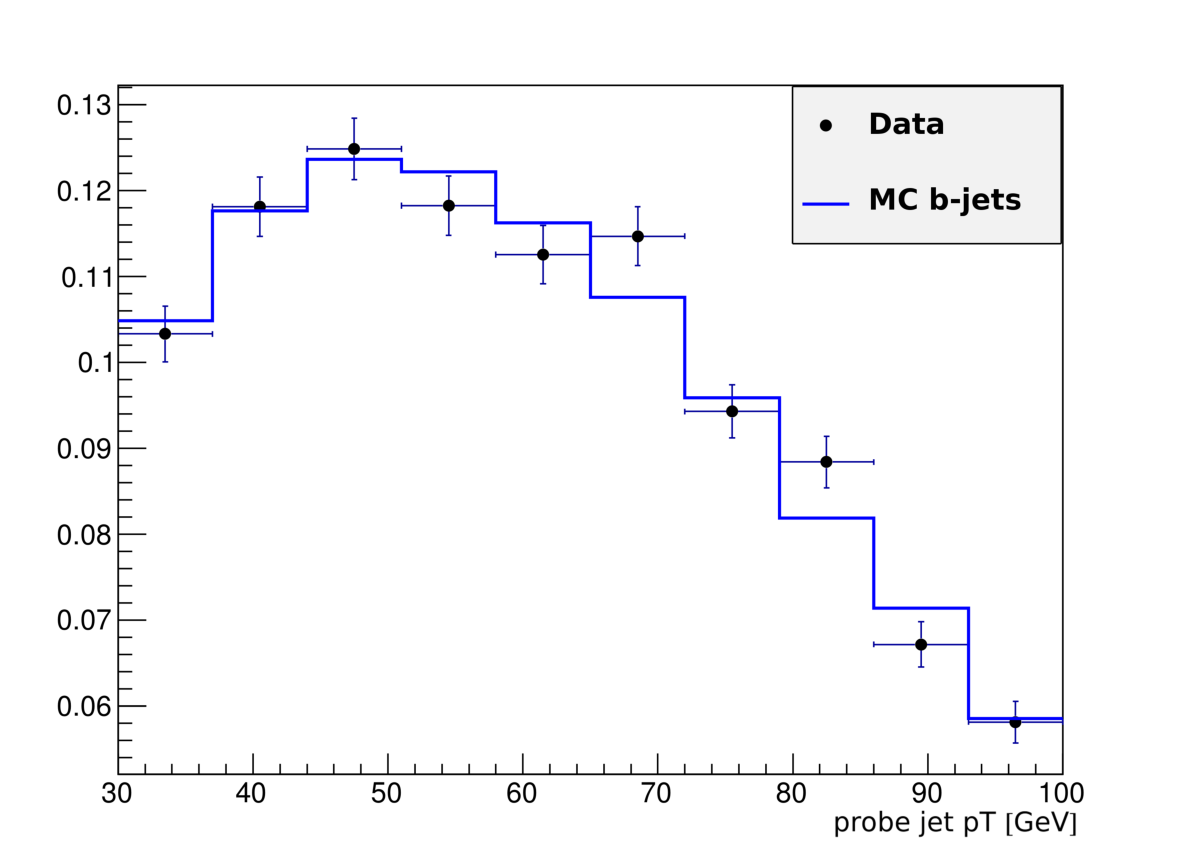
\includegraphics[width=0.6\textwidth]{images/passprobe_data_mc-v2.pdf}
\caption{Shape comparison for the \pt spectrum of the \probe jet in data and simulation in a very pure phase space enriched in b-jets.\label{fig:purett}}
\end{figure}

Finally the fit is performed using real data, as shown in Fig.~\ref{fig:data_tp}, providing the following efficiencies:
\begin{equation}
\begin{split}
\varepsilon_\mathrm{s}^\mathrm{Data} &= 0.77\pm0.02\\
\varepsilon_\mathrm{b}^\mathrm{Data} &= 0.12\pm0.05
\end{split}
\end{equation}

\begin{figure}[htb]
\centering
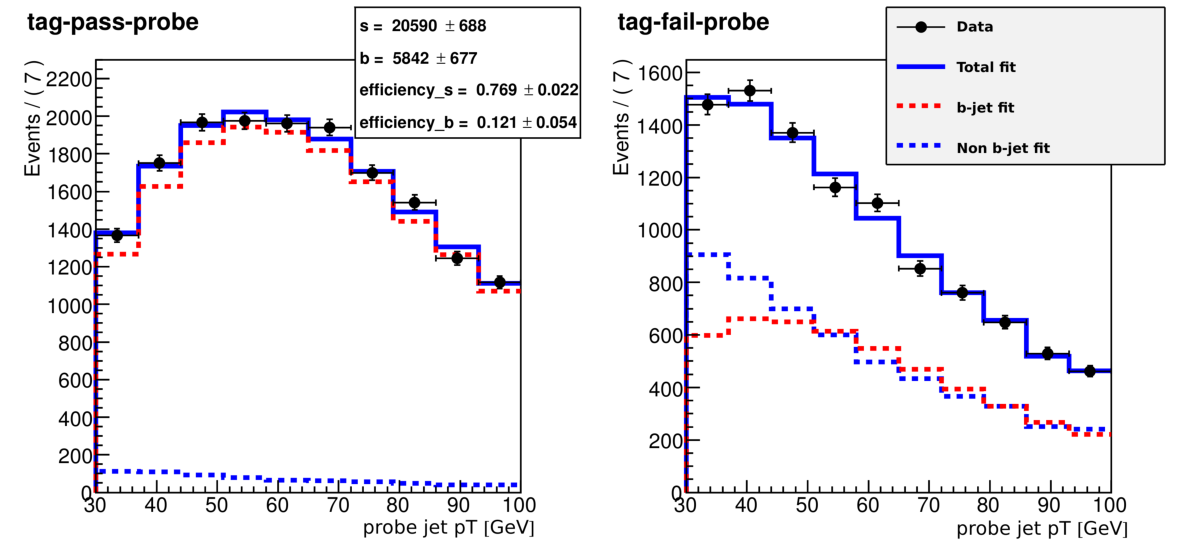
\includegraphics[width=0.8\textwidth]{images/data_ptprobe-v2.pdf}
\caption{Results of the simultaneous fit of the \tpp and \tfp pairs in the data.\label{fig:data_tp}}
\end{figure}

Further studies have been performed to assess the effect of the relative uncertainty on the \ttbar and tW event fractions. The procedure described above has been applied to different simulation templates obtained varying the \ttbar and tW fractions within theoretical uncertainties, and the effect on the parameters extracted with the fit procedure is found to be well below the fit uncertainties.

The ratio of the efficiency measured in data and simulation represents a per-jet scale factor that can be used to reweight the simulated events. The weights to be applied event-by-event depend on the particular jet configuration in the events themselves. For the signal region ($SR$), in which a b tagging veto is required, the event weight to be applied is given by:
\begin{equation}
w_{SR} = \prod_{N_\mathrm{b-jets}} \left( \frac{1-\varepsilon_\mathrm{s}^\mathrm{Data}}{1-\varepsilon_\mathrm{s}^\mathrm{MC}} \right) \prod_{N_\mathrm{non-b-jets}} \left( \frac{1-\varepsilon_\mathrm{b}^\mathrm{Data}}{1-\varepsilon_\mathrm{b}^\mathrm{MC}} \right) \quad ,
\end{equation}

\noindent where $N_\mathrm{b-jets}$ and $N_\mathrm{non-b-jets}$ are the numbers of true b-jets and non-b-jets in the simulated event, respectively. This weight is valid if the a b tagging veto is applied. If instead the b tagging veto is reverted, also the event weight has to be modified. This is done, for example, when one wants to define a \ttbar enriched control region ($CR_{\ttbar}$) for the purpose of measuring the contribution of this background in a phase space orthogonal to the signal region. One simple way to define this control region is to require the leading jet in the event to be b-tagged. Therefore, the simulated events falling in this category must be reweighted using the following weight:
\begin{equation}
w_{CR_{\ttbar}} = 
\begin{cases}
\varepsilon_\mathrm{s}^\mathrm{Data}/\varepsilon_\mathrm{s}^\mathrm{MC},& \text{if the leading jet is a b-jet} \\
\varepsilon_\mathrm{b}^\mathrm{Data}/\varepsilon_\mathrm{b}^\mathrm{MC},& \text{if the leading jet is not a b-jet} 
\end{cases}
\end{equation}




\subsection{Fiducial phase space}\label{sec:fid_space}
The Higgs boson transverse momentum is measured in a particle level fiducial phase space, whose definition is chosen in order to minimize the dependence of the measurements on the underlying model of the Higgs boson production and decay properties.

The exact requirements are determined by considering the two following correlated quantities: the reconstruction efficiency for signal events originating from within the fiducial phase space (fiducial signal efficiency $\varepsilon_{\rm{fid}}$), and the ratio of the number of reconstructed signal events that are from outside the fiducial phase space (``out-of-fiducial'' signal events) to the number from within the fiducial phase space. The requirement of having a small fraction of out-of-fiducial signal events, while at the same time preserving a high value of the fiducial signal efficiency $\epsilon_{\rm{fid}}$, leads to fiducial requirements at the generator level on the low-resolution variables, \MET and \mt, that are looser with respect to those applied in the reconstructed event selection.

The fiducial phase space used for the cross section measurements is defined at the particle level by the requirements given in Table~\ref{table:fid_cuts}. The leptons are defined as Born-level leptons, i.e. before the emission of final-state radiation (FSR), and are required not to  originate from leptonic $\tau$ decays. The effect of including FSR is found to modify $\epsilon_{\rm{fid}}$ at most of about 5\%.
For the VH signal process, the two leptons are required to originate from the \hwwllnn decays in order to avoid including leptons coming from the associated W or Z boson.

\begin{table}[htb]
\caption{Summary of requirements used in the definition of the fiducial phase space.}\label{table:fid_cuts}
\begin{center}
\begin{tabular}{l r}
\toprule
\bf{Physics quantity} & \bf{Requirement} \\
\midrule
Leading lepton \pt & $\pt > 20$\GeV \\
Subleading lepton \pt & $\pt > 10$\GeV \\
Pseudorapidity of electrons and muons & $|\eta| < 2.5$ \\
Invariant mass of the two charged leptons & $\mll > 12$\GeV \\
Charged lepton pair \pt & $p_{\rm T}^{\ell\ell} > 30$\GeV \\
Invariant mass of the leptonic system in the transverse plane & $m_{\rm T}^{\ell\ell \nu\nu} > 50$\GeV \\
\MET & $\MET>0$ \\
\bottomrule
\end{tabular}
\end{center}
\end{table}

A detailed description of the fiducial region definition and its optimization is given in Appendix~\ref{app:fiducial_region}.










\subsection{Binning of the \pth distribution}

Experimentally, the Higgs boson transverse momentum is reconstructed as the vector sum of the lepton momenta in the transverse plane and \ptmiss.
\begin{equation}
\vec{p}_\mathrm{T}^\mathrm{~H} = \vec{p}_\mathrm{T}^{~\ell\ell} + \vec{p}_\mathrm{T}^\mathrm{~miss}
\end{equation}
Compared to other differential analyses of the Higgs boson cross section, such as those in the ZZ and $\gamma\gamma$ decay channels, this analysis has to cope with the limited resolution due to the \MET entering the transverse momentum measurement.
The effect of the limited \MET resolution has two main implications on the analysis strategy: the first one is that the choice of the binning of the \pth{} spectrum needs to take into account the detector resolution; the second implication is that migrations of events across bins are significant and an unfolding procedure needs to be applied to correct for selection efficiencies and bin migration effects.

Given these aspects, the criterion that is used to define the \pth bin size is devised to keep under control the bin migrations due to the finite resolution.
For any given bin $i$, the purity $P_i$ of the signal sample is defined as the number of events that are generated and also reconstructed in that bin, $N_i^\mathrm{GEN|RECO}$, divided by the number of events reconstructed in the same bin, $N_i^\mathrm{RECO}$:
\begin{equation}\label{eq:purity}
P_i = \frac{N_i^\mathrm{GEN|RECO}}{N_i^\mathrm{RECO}} \quad .
\end{equation}

The bin width is chosen in such a way as to make the smallest bins able to ensure a purity of about 60\%, based on a ggH simulated sample.
Following this prescription, the whole \pth range is divided in the following six bins: \mbox{[0--15]\GeV}, \mbox{[15--45]\GeV}, \mbox{[45--85]\GeV}, \mbox{[85--125]\GeV}, \mbox{[125--165]\GeV}, \mbox{[165--$\infty$]\GeV}.

The fiducial signal efficiency $\varepsilon_\mathrm{fid}$ and the fraction of out-of-fiducial signal events, $f_{\text{out-of-fid}}$, are different in each \pth bin and depend on the definition of the fiducial phase space. In Fig.~\ref{fig:sel_eff} the $\varepsilon_\mathrm{fid}$ and $f_{\text{out-of-fid}}$ parameters are shown in each \pth bin for different definitions of the fiducial phase space. In particular, they have been evaluated adding the requirements reported in Table~\ref{table:fid_cuts} in sequence, starting from a fiducial phase space defined just by the lepton \pt and $\eta$ selections, together with the different flavour requirement, and adding each time an additional selection until the full fiducial phase space in obtained. In this way, the effect of every single selection (or group of selections) on $\varepsilon_\mathrm{fid}$ and $f_{\text{out-of-fid}}$ can be assessed. Since the variables related to leptons are measured with good resolution, the effect of including the lepton selections in the fiducial phase space is to increase $\varepsilon_\mathrm{fid}$ keeping $f_{\text{out-of-fid}}$ constant. Instead, the effect of including low-resolution variables, such as \mt, is to increase both $\varepsilon_\mathrm{fid}$ and $f_{\text{out-of-fid}}$. Nevertheless, the $f_{\text{out-of-fid}}$ parameter is different from zero even if only lepton selections are taken into account. This is ascribable to two different aspects: the first one is that in the fiducial phase space electrons and muons are required not to originate from $\tau$ decays; the second one is instead related to the VH production mechanism, i.e. to the fact that leptons coming from the associated boson are not included.

%The efficiency of the analysis selection with respect to the fiducial phase space is reported in Fig.~\ref{fig:sel_eff} (a) for each \pth bin. The efficiency denominator is the number of events that are inside the fiducial phase space, while the numerator is the number of events that pass both the analysis and the fiducial phase space selections. The fake rate, defined by the ratio of signal events that pass the analysis selection but are not within the fiducial phase space, divided by the total number of events passing both the analysis and the fiducial phase space selections is shown in Fig.~\ref{fig:sel_eff} (b). For both the selection efficiency and the fake rate, all the signal production mechanisms are included.
The overall values obtained integrating over \pth are $\varepsilon_\mathrm{fid}=0.362\pm{0.005}$ and $f_{\text{out-of-fid}}=0.126\pm0.004$ respectively, where only statistical uncertainties are taken into account.

\begin{figure}[htb]
\centering
\subfigure[]{
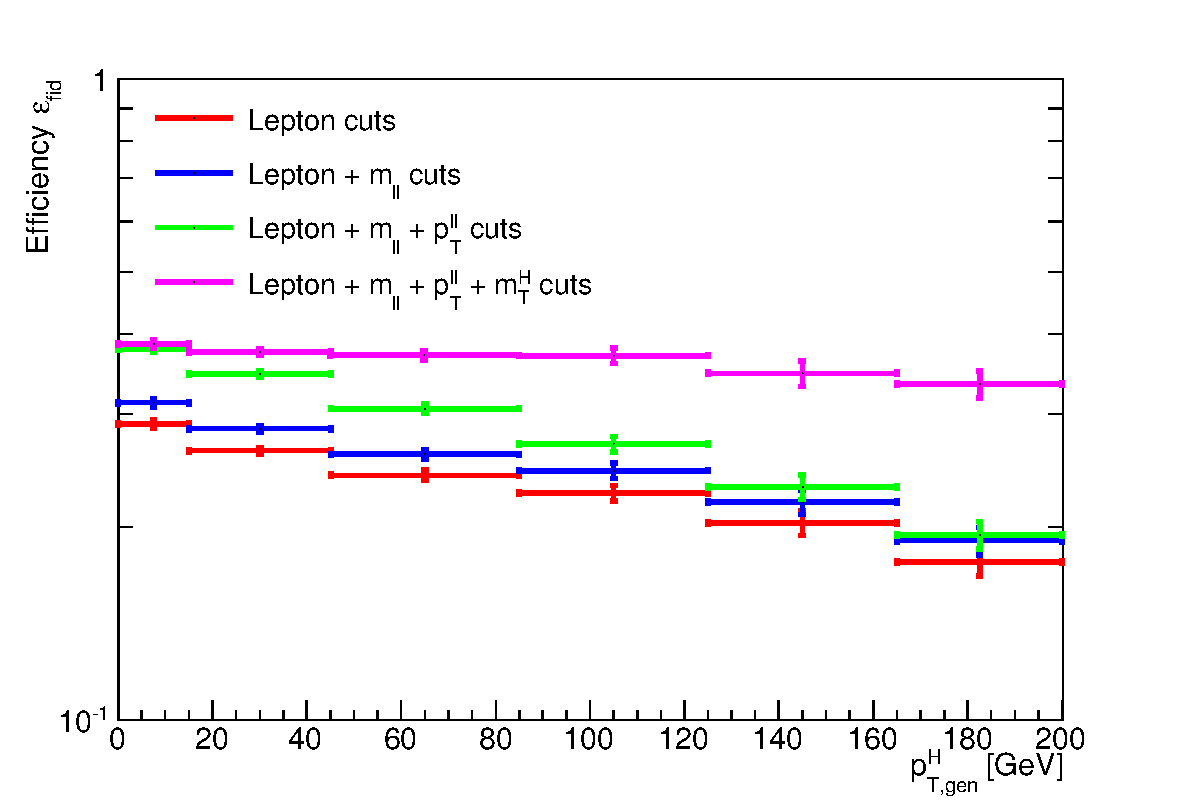
\includegraphics[width=0.45\textwidth]{images/eff-fid.pdf}
}
\subfigure[]{
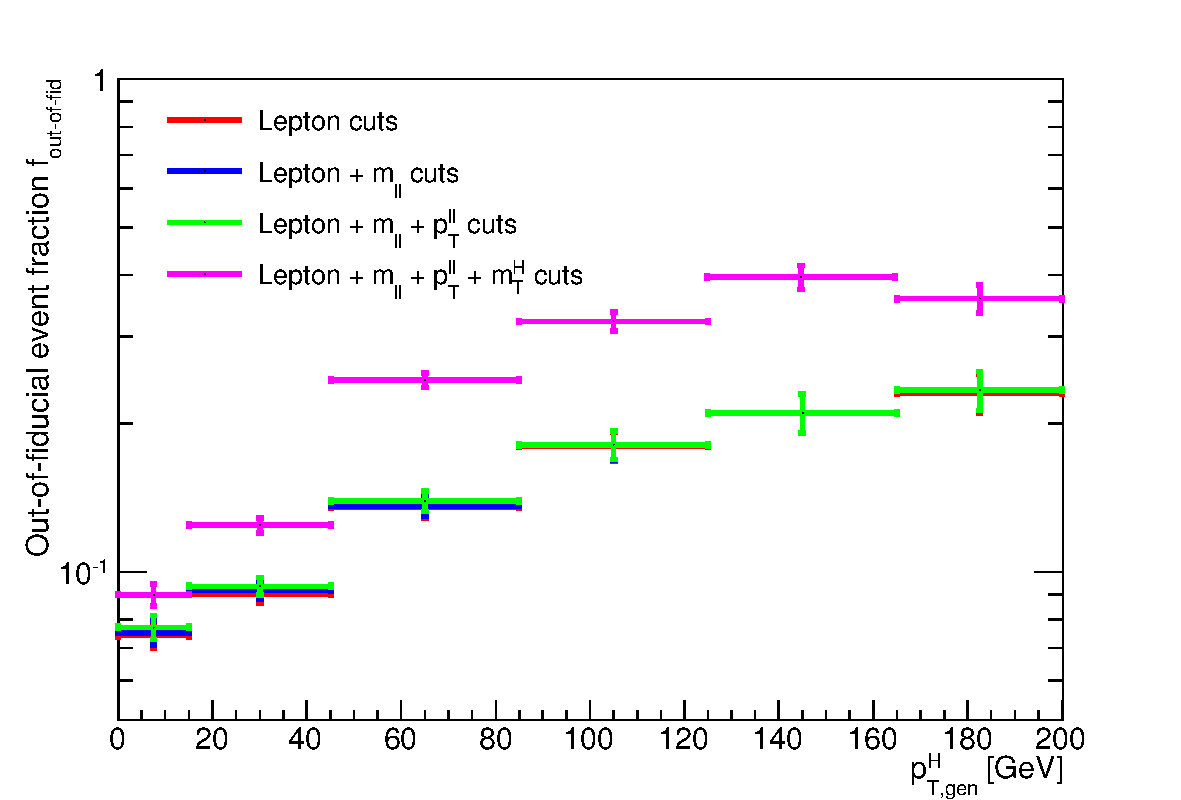
\includegraphics[width=0.45\textwidth]{images/out-of-fid.pdf}
}
\caption{Fiducial signal efficiency $\varepsilon_\mathrm{fid}$ and fraction of out-of-fiducial signal events $f_{\text{out-of-fid}}$ in each bin of the generator level \pth.\label{fig:sel_eff}}
\end{figure}

If a wider acceptance is defined, only requiring that the Higgs boson decays to WW and then to $2\ell2\nu$, the efficiency becomes $\epsilon=0.0396\pm{0.0003}$ and the fraction of out-of-fiducial signal events is zero. 





